\begin{comment}
\section{Osservabili stellari/demo beamer}
\begin{frame}<1>[label=noinside]{Modello stellare}{Come indagare la fisica interna a una stella?}
\onslide<1->\begin{block}{Osservabili stellari:}
$L$, $M$, $R$, $T_e$, $(\frac{Z}{X})_{ph}$, $g_{ph}$.
\end{block}
\onslide<1->\begin{block}{Informazioni sulla struttura interna?} Condizione di equilibrio idrostatico
\end{block}
%Teorema Vogt-Russel: $X_i(r)$, $M$ \pause equilibrio (idrostatico/termico) determinano struttura stellare .
%\pause
\onslide<1->\begin{block}{Modello stellare: diagramma di \hr{}.}
\end{block}
\onslide<2->\begin{block}{Descrizione fisica interno stellare: parametri aggiuntivi}
Convezione, diffusione e sedimentazione elementi pesanti, equazione di stato, opacit\'a
\end{block}
\onslide<2->\begin{block}{Astrosismologia}
Restringo spazio parametri sistemi stellari lontani
\end{block}
\end{frame}
{ % all template changes are local to this group.
\setbeamertemplate{navigation symbols}{}
    \begin{frame}[plain]{Diagramma di \hr{}}
        \begin{tikzpicture}[remember picture,overlay]
            \node[at=(current page.center)] {
                %\includegraphics[width=\paperwidth]{yourimage}
            };
        \end{tikzpicture}
     \end{frame}
}
\againframe<2>{noinside}
\section{Osservazioni}
\subsection{Fitting polinomiale: inversione ''1.5-D''.}
\begin{frame}<1>[label=noinside]{Modello stellare}{Come indagare la fisica interna a una stella?}
\onslide<1->\begin{block}{Rotazione superficiale}
\begin{equation*}
\frac{\Omega(\theta)}{2\pi}=\SI{451.5}{\nano\hertz}-\SI{65.3}{\nano\hertz}\cos^2{\theta}-\SI{66.7}{\nano\hertz}\cos^4{\theta}
\end{equation*}
\end{block}
\onslide<1->\begin{block}{Informazioni sulla struttura interna?} Condizione di equilibrio idrostatico
\end{block}
%Teorema Vogt-Russel: $X_i(r)$, $M$ \pause equilibrio (idrostatico/termico) determinano struttura stellare .
%\pause
\onslide<1->\begin{block}{Modello stellare: diagramma di \hr{}.}
\end{block}
\onslide<2->\begin{block}{Descrizione fisica interno stellare: parametri aggiuntivi}
Convezione, diffusione e sedimentazione elementi pesanti, equazione di stato, opacit\'a
\end{block}
\onslide<2->\begin{block}{Astrosismologia}
Restringo spazio parametri sistemi stellari lontani
\end{block}
\end{frame}
\subsection{Osservazione dello splitting in m: inversione ''2D''.}
\begin{figure}[!ht]
\centering
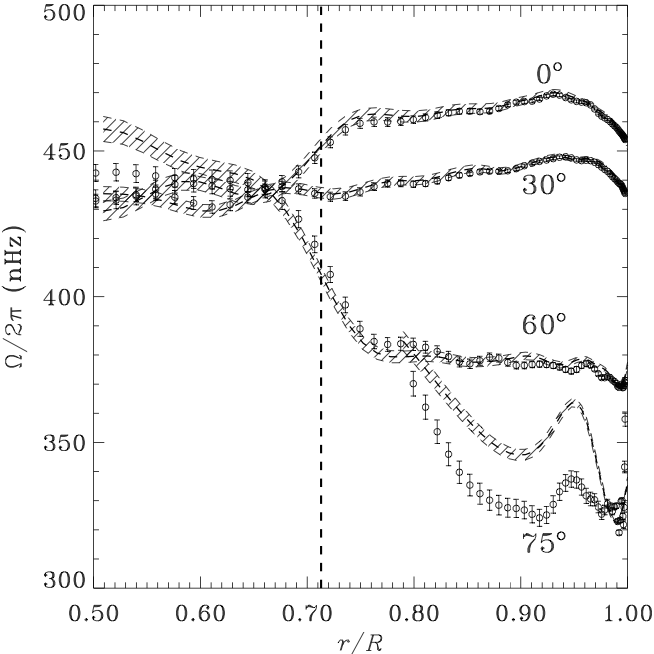
\includegraphics[keepaspectratio,width=0.8\textwidth]{invertedrotation}
\caption{Inversione della velocit\'a di rotazione a diverse latitudini. La linea verticale tratteggiata indica la base della zona convettiva. Da \cite{chr02helioseismology}.}
\end{figure}
Considero la correzione al primo ordine in $\Omega$. Il campo di velocit\'a rotazionale in coordinate sferiche \'e 
\begin{align}
&\vec{v_0}=(0,0,r\Omega\sin{\theta})=\vecp{\Omega}{r}\\
&\vec{\Omega(r,\theta)}=(\Omega(r,\theta)\cos{\theta},-\Omega(r,\theta)\sin{\theta},0)
\end{align}
In assenza di moti macroscopici il termine d'inerzia \'e $\rho_0\TDy{t}{\vec{v}}=\rho_0\PtwoDy{t}{\vec{\xi}}$, mentre in caso di rotazione si ha
\begin{equation}
\rho_0(\PDof{t}+\scap{v_0}{\nabla})^2\vec{\xi}
\end{equation}
Considero il termine dovuto alla rotazione come una piccola correzione alle frequenze dei modi
\begin{align}
&\omega_{(l,m)}+\Delta\omega_{(l,m)}&\intertext{quindi l'equazione del moto al primo ordine nella perturbazione, con $\alpha=(l,m)$, \'e}\nonumber\\
&\rho_0(\omega_{\alpha}^2+2\omega_{\alpha}\Delta\omega_{\alpha})\vec{\xi}=\nabla P_1-\frac{\rho_1}{\rho_0}\nabla P_0+\rho_0\nabla\Phi_1+2i\omega_{\alpha}\rho_0(\scap{v_0}{\nabla})\vec{\xi}\\
&\intertext{da cui si deduce}\nonumber\\
&\Delta\omega_{\alpha}=\frac{i\int\rho_0\xi_{\alpha}^*(\scap{v_0}{\nabla})\xi_{\alpha}}{\int\rho_0\xi_{\alpha}^*\xi_{\alpha}}=\frac{-m\int\rho_0\Omega\xi_{\alpha}^*\xi_{\alpha}\,dV+i\int\rho_0\xi_{\alpha}^*(\vecp{\Omega}{\xi_{\alpha}})\,dV}{\int\rho_0\xi_{\alpha}^*\xi_{\alpha}}
\end{align}
Il problema di trovare $\Omega(r,\theta)$ dalla differenza $\Delta\omega_{\alpha}$ \'e lineare in $\Omega$ quindi $\Delta\omega_{\alpha}\propto\Omega$. Per determinare quindi la rotazione dobbiamo conoscere l'autovalore $\xi_{\alpha}$ dello stato imperturbato.
%Per rotazione puramente radiale $\Omega(r)$ la relazione tra lo splitting delle frequenze e la rotazione \'e
%\begin{equation}
%\Delta\omega_{\alpha}=-m\frac{\int_0^{\rsun{}}\rho_0\Omega\{|\xi_r-\xi_h|^2+[l(l+1)-2]|\xi_h|^2\}r^2\,dr}{\int_0^{\rsun{}}\rho_0\{|\xi_r|^2+l(l+1)|\xi_h|^2\}r^2\,dr}=\int_0^{\rsun{}}K_{\alpha}(r)\Omega(r)\,dr
%\end{equation}
%Any given $\Delta\omega_{\alpha}$ samples angular velocity in the depth range corresponding to $\xi_{\alpha}$.
La velocit\'a angolare contribuisce a $\Delta\omega_{\alpha}$ negli strati in cui $\xi_{\alpha}$ \'e apprezzabile. Nel caso di rotazione dipendente solo da r si ha che $\Delta\omega_{\alpha}$ \'e lineare in m: ho $2l+1$ frequenze equispaziate.

\end{comment}

\section{Modi normali della struttura solare}

\begin{frame}[label=noinside]{Modi di oscillazione adiabatici}{Perturbazione dello stato di equilibrio.}

\begin{block}{campi di velocit\'a/effetti non lineari}
Descrivo le oscillazioni come piccole perturbazioni attorno allo stato di equilibrio stazionario (gli effetti non lineari, fra cui lo scambio di energia tra i modi, sono dell'ordine di $\frac{v}{c_s}$ dove v \'e l'ampiezza della velocit\'a dell'oscillazione). 
In generale pu\'o essere presente un campo di velocit\'a $\vec{v}_0$:
\begin{align}
&\vec{v}=\vec{v}_0+\vec{v}'\\
&\TDof{t}=\PDof{t}+(\vec{v}_0\cdot\nabla)
\end{align}
in prima approssimazione prendo $\vec{v}_0=0$ per poi considerare come perturbazioni gli effetti dovuti a campi di velocit\'a in specie rotazione.

\end{block}

\begin{block}{Perturbazione pressione densit\'a}

Indico con $P'(\vec{r},t)$ e $\delta P$ la perturbazione euleriana e lagrangiana della pressione e con $\rho'$, $\Phi'$ e $\vec{g}'$ la perturbazione euleriana della densit\'a , e le perturbazioni euleriane del potenziale gravitazionale e dell'accelerazione di gravit\'a conseguenti  con $\delta\vec{r}=\vec{\xi}$ il vettore spostamento perturbato:
\begin{align}
&P(\vec{r},t)=P_0(\vec{r})+P'(\vec{r},t)\label{eq:pressureperturbation}\\
&\Lvar{P(\vec{r})}=P(\vec{r}+\Lvar{\vec{r}})-P_0(\vec{r})=P'(\vec{r})+\Lvar{\vec{r}}\cdot\nabla P_0\\
&\vec{g}'=-\nabla\Phi',\ \nabla^2\Phi'=4\pi G\rho'\label{eq:gapert}
\end{align}

\end{block}


\end{frame}

\begin{frame}[label=noinside]{Modi di oscillazione adiabatici}{Modi di oscillazione lineari adiabatici.}

\begin{block}{Equazione del moto perturbata}

l'equazione del moto perturbato sostituendo \eqref{eq:pressureperturbation} nell'equazione del moto \eqref{eq:motion} considerando solo i termini lineari nella perturbazione:
\begin{equation}
\rho_0\TDof{t}\vec{v}=\rho_0\PtwoDy{t}{\Lvar{\vec{r}}}=-\nabla P'+\rho_0\vec{g}'+\rho'\vec{g}_0\label{eq:emper}
\end{equation}

\end{block}

\end{frame}

\begin{frame}[label=noinside]{Modi di oscillazione adiabatici}{Equazione di continuit\'a perturbata}

\begin{block}{Equazione di continuit\'a perturbata}

Analogamente per l'equazione di continuit\'a ottengo
\begin{equation}
\rho'+\div{(\rho_0\Lvar{\vec{r}})}=0\label{eq:contper}
\end{equation}

\end{block}

\end{frame}

\begin{frame}[label=noinside]{Modi di oscillazione adiabatici}{Condizione di adiabaticit\'a}


  \begin{overlayarea}{\textwidth}{1cm}
   \only<1>{
   energia interna per unit\'a di massa
\begin{equation}
\TDy{t}{q}=\TDy{t}{u}+P\TDof{t}(\frac{1}{\rho})\label{eq:prima}
\end{equation}

\begin{equation}
\TDy{t}{T}-\frac{\Gamma_2-1}{\Gamma_2}\frac{T}{P}\TDy{t}{P}=\frac{1}{c_P}(\epsilon-\frac{1}{\rho}\scap{\nabla}{F})
\end{equation}
il termine a destra \'e trascurabile:
\begin{equation}
\TDy{t}{q}=0
\end{equation}
   }
   \only<2>{
   Il moto di una elemento di fluido \'e descritto dalla relazione adiabatica
\begin{equation}
\TDy{t}{P}=\frac{\Gamma_1P}{\rho}\TDy{t}{\rho}
\end{equation}
}
   \only<3>{
  
  La condizione di perturbazione adiabatica linearizzata \'e
\begin{align}
&\PDy{t}{\Lvar{P}}-\frac{\Gamma_{1,0}P_0}{\rho_0}\PDy{t}{\Lvar{\rho}}=0\\
&P'+\Lvar{\vec{\xi}}\cdot\nabla P_0=\frac{\Gamma_{1,0}P_0}{\rho}(\rho'+\Lvar{\vec{\xi}}\cdot\nabla\rho_0)\label{eq:adper}
\end{align}

   }
  \end{overlayarea}


\end{frame}


\begin{figure}[!ht]

\subfigure[Distribuzione dei modi con $l\leq300$ nel diagramma $\nu-l$ determinata usando i primi 144 giorni di osservazione di MDI. Da \cite{chr02helioseismology}.]{
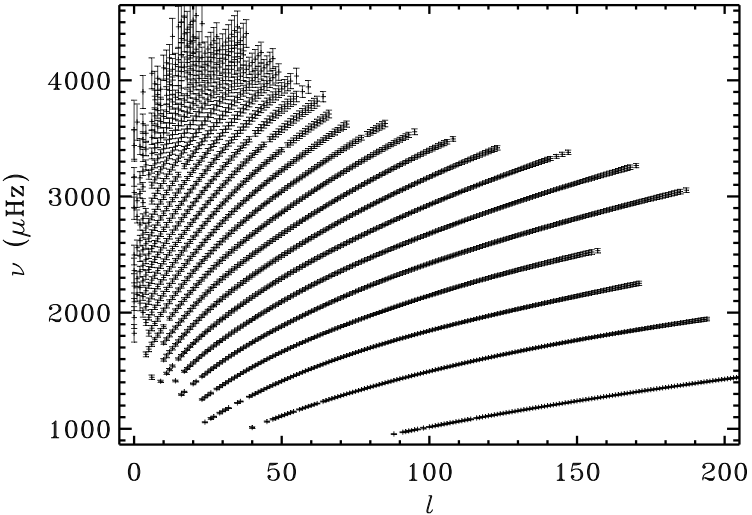
\includegraphics[keepaspectratio,width=0.45\textwidth]{midlmodes}}
\label{fig:midlmodes}
~
\subfigure[Modi adiabatici calcolati sulla base di un modello solare. Da \cite{chr02helioseismology}.]{
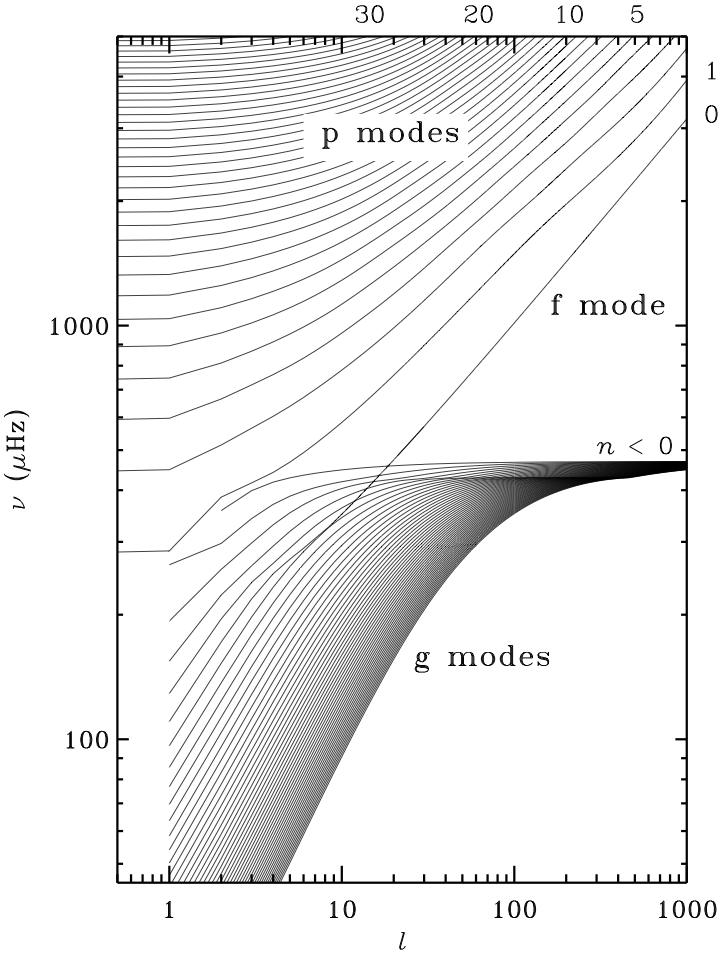
\includegraphics[keepaspectratio,width=0.6\textwidth]{nrmodesLAWE}\label{fig:nrmodesLAWE}}

\end{figure}

\section{Campo di velocit\'a solare}

\section{Caratteristiche asintotiche delle oscillazioni adiabatiche}

